% Options for packages loaded elsewhere
\PassOptionsToPackage{unicode}{hyperref}
\PassOptionsToPackage{hyphens}{url}
%
\documentclass[
]{article}
\usepackage{amsmath,amssymb}
\usepackage{iftex}
\ifPDFTeX
  \usepackage[T1]{fontenc}
  \usepackage[utf8]{inputenc}
  \usepackage{textcomp} % provide euro and other symbols
\else % if luatex or xetex
  \usepackage{unicode-math} % this also loads fontspec
  \defaultfontfeatures{Scale=MatchLowercase}
  \defaultfontfeatures[\rmfamily]{Ligatures=TeX,Scale=1}
\fi
\usepackage{lmodern}
\ifPDFTeX\else
  % xetex/luatex font selection
\fi
% Use upquote if available, for straight quotes in verbatim environments
\IfFileExists{upquote.sty}{\usepackage{upquote}}{}
\IfFileExists{microtype.sty}{% use microtype if available
  \usepackage[]{microtype}
  \UseMicrotypeSet[protrusion]{basicmath} % disable protrusion for tt fonts
}{}
\makeatletter
\@ifundefined{KOMAClassName}{% if non-KOMA class
  \IfFileExists{parskip.sty}{%
    \usepackage{parskip}
  }{% else
    \setlength{\parindent}{0pt}
    \setlength{\parskip}{6pt plus 2pt minus 1pt}}
}{% if KOMA class
  \KOMAoptions{parskip=half}}
\makeatother
\usepackage{xcolor}
\usepackage[margin=1in]{geometry}
\usepackage{color}
\usepackage{fancyvrb}
\newcommand{\VerbBar}{|}
\newcommand{\VERB}{\Verb[commandchars=\\\{\}]}
\DefineVerbatimEnvironment{Highlighting}{Verbatim}{commandchars=\\\{\}}
% Add ',fontsize=\small' for more characters per line
\usepackage{framed}
\definecolor{shadecolor}{RGB}{248,248,248}
\newenvironment{Shaded}{\begin{snugshade}}{\end{snugshade}}
\newcommand{\AlertTok}[1]{\textcolor[rgb]{0.94,0.16,0.16}{#1}}
\newcommand{\AnnotationTok}[1]{\textcolor[rgb]{0.56,0.35,0.01}{\textbf{\textit{#1}}}}
\newcommand{\AttributeTok}[1]{\textcolor[rgb]{0.13,0.29,0.53}{#1}}
\newcommand{\BaseNTok}[1]{\textcolor[rgb]{0.00,0.00,0.81}{#1}}
\newcommand{\BuiltInTok}[1]{#1}
\newcommand{\CharTok}[1]{\textcolor[rgb]{0.31,0.60,0.02}{#1}}
\newcommand{\CommentTok}[1]{\textcolor[rgb]{0.56,0.35,0.01}{\textit{#1}}}
\newcommand{\CommentVarTok}[1]{\textcolor[rgb]{0.56,0.35,0.01}{\textbf{\textit{#1}}}}
\newcommand{\ConstantTok}[1]{\textcolor[rgb]{0.56,0.35,0.01}{#1}}
\newcommand{\ControlFlowTok}[1]{\textcolor[rgb]{0.13,0.29,0.53}{\textbf{#1}}}
\newcommand{\DataTypeTok}[1]{\textcolor[rgb]{0.13,0.29,0.53}{#1}}
\newcommand{\DecValTok}[1]{\textcolor[rgb]{0.00,0.00,0.81}{#1}}
\newcommand{\DocumentationTok}[1]{\textcolor[rgb]{0.56,0.35,0.01}{\textbf{\textit{#1}}}}
\newcommand{\ErrorTok}[1]{\textcolor[rgb]{0.64,0.00,0.00}{\textbf{#1}}}
\newcommand{\ExtensionTok}[1]{#1}
\newcommand{\FloatTok}[1]{\textcolor[rgb]{0.00,0.00,0.81}{#1}}
\newcommand{\FunctionTok}[1]{\textcolor[rgb]{0.13,0.29,0.53}{\textbf{#1}}}
\newcommand{\ImportTok}[1]{#1}
\newcommand{\InformationTok}[1]{\textcolor[rgb]{0.56,0.35,0.01}{\textbf{\textit{#1}}}}
\newcommand{\KeywordTok}[1]{\textcolor[rgb]{0.13,0.29,0.53}{\textbf{#1}}}
\newcommand{\NormalTok}[1]{#1}
\newcommand{\OperatorTok}[1]{\textcolor[rgb]{0.81,0.36,0.00}{\textbf{#1}}}
\newcommand{\OtherTok}[1]{\textcolor[rgb]{0.56,0.35,0.01}{#1}}
\newcommand{\PreprocessorTok}[1]{\textcolor[rgb]{0.56,0.35,0.01}{\textit{#1}}}
\newcommand{\RegionMarkerTok}[1]{#1}
\newcommand{\SpecialCharTok}[1]{\textcolor[rgb]{0.81,0.36,0.00}{\textbf{#1}}}
\newcommand{\SpecialStringTok}[1]{\textcolor[rgb]{0.31,0.60,0.02}{#1}}
\newcommand{\StringTok}[1]{\textcolor[rgb]{0.31,0.60,0.02}{#1}}
\newcommand{\VariableTok}[1]{\textcolor[rgb]{0.00,0.00,0.00}{#1}}
\newcommand{\VerbatimStringTok}[1]{\textcolor[rgb]{0.31,0.60,0.02}{#1}}
\newcommand{\WarningTok}[1]{\textcolor[rgb]{0.56,0.35,0.01}{\textbf{\textit{#1}}}}
\usepackage{graphicx}
\makeatletter
\def\maxwidth{\ifdim\Gin@nat@width>\linewidth\linewidth\else\Gin@nat@width\fi}
\def\maxheight{\ifdim\Gin@nat@height>\textheight\textheight\else\Gin@nat@height\fi}
\makeatother
% Scale images if necessary, so that they will not overflow the page
% margins by default, and it is still possible to overwrite the defaults
% using explicit options in \includegraphics[width, height, ...]{}
\setkeys{Gin}{width=\maxwidth,height=\maxheight,keepaspectratio}
% Set default figure placement to htbp
\makeatletter
\def\fps@figure{htbp}
\makeatother
\setlength{\emergencystretch}{3em} % prevent overfull lines
\providecommand{\tightlist}{%
  \setlength{\itemsep}{0pt}\setlength{\parskip}{0pt}}
\setcounter{secnumdepth}{-\maxdimen} % remove section numbering
\ifLuaTeX
  \usepackage{selnolig}  % disable illegal ligatures
\fi
\IfFileExists{bookmark.sty}{\usepackage{bookmark}}{\usepackage{hyperref}}
\IfFileExists{xurl.sty}{\usepackage{xurl}}{} % add URL line breaks if available
\urlstyle{same}
\hypersetup{
  hidelinks,
  pdfcreator={LaTeX via pandoc}}

\author{}
\date{\vspace{-2.5em}}

\begin{document}

\hypertarget{image-processing-word-cloud-and-network-analysis}{%
\section{Image Processing, Word Cloud, and Network
Analysis}\label{image-processing-word-cloud-and-network-analysis}}

\hypertarget{mahdiyeh-ebrahimy}{%
\subsection{Mahdiyeh Ebrahimy}\label{mahdiyeh-ebrahimy}}

\textbf{Student ID:} 4011290481

\begin{center}\rule{0.5\linewidth}{0.5pt}\end{center}

\hypertarget{table-of-contents}{%
\subsection{Table of Contents}\label{table-of-contents}}

\begin{enumerate}
\def\labelenumi{\arabic{enumi}.}
\tightlist
\item
  \protect\hyperlink{image-processing}{Image Processing}\\
\item
  \protect\hyperlink{word-cloud}{Word Cloud}\\
\item
  \protect\hyperlink{network-analysis}{Network Analysis}
\end{enumerate}

\begin{center}\rule{0.5\linewidth}{0.5pt}\end{center}

\hypertarget{image-processing}{%
\subsection{Image Processing}\label{image-processing}}

\hypertarget{code}{%
\subsubsection{Code}\label{code}}

\begin{Shaded}
\begin{Highlighting}[]
\FunctionTok{options}\NormalTok{(}\AttributeTok{warn =} \SpecialCharTok{{-}}\DecValTok{1}\NormalTok{)}
\FunctionTok{library}\NormalTok{(ggplot2)}
\FunctionTok{library}\NormalTok{(grid)}
\FunctionTok{library}\NormalTok{(magick)}
\end{Highlighting}
\end{Shaded}

\begin{verbatim}
## Linking to ImageMagick 6.9.12.98
## Enabled features: cairo, freetype, fftw, ghostscript, heic, lcms, pango, raw, rsvg, webp
## Disabled features: fontconfig, x11
\end{verbatim}

\begin{Shaded}
\begin{Highlighting}[]
\NormalTok{image\_path }\OtherTok{\textless{}{-}} \StringTok{"ShowPic.png"}

\NormalTok{original\_image }\OtherTok{\textless{}{-}} \FunctionTok{image\_read}\NormalTok{(image\_path)}

\CommentTok{\# Resize and process image}
\NormalTok{resized\_image }\OtherTok{\textless{}{-}} \FunctionTok{image\_scale}\NormalTok{(original\_image, }\StringTok{"600x400"}\NormalTok{)}
\NormalTok{image\_width }\OtherTok{\textless{}{-}} \FunctionTok{as.numeric}\NormalTok{(}\FunctionTok{image\_info}\NormalTok{(resized\_image)}\SpecialCharTok{$}\NormalTok{width)}
\NormalTok{image\_height }\OtherTok{\textless{}{-}} \FunctionTok{as.numeric}\NormalTok{(}\FunctionTok{image\_info}\NormalTok{(resized\_image)}\SpecialCharTok{$}\NormalTok{height)}
\NormalTok{left\_half }\OtherTok{\textless{}{-}} \FunctionTok{image\_crop}\NormalTok{(resized\_image, }\FunctionTok{paste0}\NormalTok{(image\_width }\SpecialCharTok{/} \DecValTok{2}\NormalTok{, }\StringTok{"x"}\NormalTok{, image\_height, }\StringTok{"+0+0"}\NormalTok{))}
\NormalTok{right\_half }\OtherTok{\textless{}{-}} \FunctionTok{image\_crop}\NormalTok{(resized\_image, }\FunctionTok{paste0}\NormalTok{(image\_width }\SpecialCharTok{/} \DecValTok{2}\NormalTok{, }\StringTok{"x"}\NormalTok{, image\_height, }\StringTok{"+"}\NormalTok{, image\_width }\SpecialCharTok{/} \DecValTok{2}\NormalTok{, }\StringTok{"+0"}\NormalTok{))}
\NormalTok{right\_half }\OtherTok{\textless{}{-}} \FunctionTok{image\_convert}\NormalTok{(right\_half, }\AttributeTok{colorspace =} \StringTok{"gray"}\NormalTok{)}
\NormalTok{combined\_image }\OtherTok{\textless{}{-}} \FunctionTok{image\_append}\NormalTok{(}\FunctionTok{c}\NormalTok{(left\_half, right\_half), }\AttributeTok{stack =} \ConstantTok{FALSE}\NormalTok{)}
\CommentTok{\#i just dont have any pic}
\NormalTok{final\_image }\OtherTok{\textless{}{-}} \FunctionTok{image\_annotate}\NormalTok{(combined\_image, }\StringTok{"Half sigma"}\NormalTok{, }\AttributeTok{size =} \DecValTok{35}\NormalTok{, }\AttributeTok{gravity =} \StringTok{"north"}\NormalTok{, }\AttributeTok{color =} \StringTok{"white"}\NormalTok{, }\AttributeTok{boxcolor =} \StringTok{"black"}\NormalTok{)}
\FunctionTok{image\_write}\NormalTok{(final\_image, }\AttributeTok{path =} \StringTok{"processed\_image.png"}\NormalTok{, }\AttributeTok{format =} \StringTok{"png"}\NormalTok{)}
\NormalTok{knitr}\SpecialCharTok{::}\FunctionTok{include\_graphics}\NormalTok{(}\StringTok{"processed\_image.png"}\NormalTok{)}
\end{Highlighting}
\end{Shaded}


\includegraphics[width=4.33in]{processed_image}

\begin{Shaded}
\begin{Highlighting}[]
\CommentTok{\# پردازش تصاویر RGB و ایجاد انیمیشن}
\NormalTok{resized\_image }\OtherTok{\textless{}{-}} \FunctionTok{image\_scale}\NormalTok{(original\_image, }\StringTok{"600x400"}\NormalTok{)}
\NormalTok{r\_image }\OtherTok{\textless{}{-}} \FunctionTok{image\_modulate}\NormalTok{(resized\_image, }\AttributeTok{brightness =} \DecValTok{100}\NormalTok{, }\AttributeTok{saturation =} \DecValTok{100}\NormalTok{, }\AttributeTok{hue =} \DecValTok{0}\NormalTok{)}
\NormalTok{g\_image }\OtherTok{\textless{}{-}} \FunctionTok{image\_modulate}\NormalTok{(resized\_image, }\AttributeTok{brightness =} \DecValTok{100}\NormalTok{, }\AttributeTok{saturation =} \DecValTok{100}\NormalTok{, }\AttributeTok{hue =} \DecValTok{120}\NormalTok{)}
\NormalTok{b\_image }\OtherTok{\textless{}{-}} \FunctionTok{image\_modulate}\NormalTok{(resized\_image, }\AttributeTok{brightness =} \DecValTok{100}\NormalTok{, }\AttributeTok{saturation =} \DecValTok{100}\NormalTok{, }\AttributeTok{hue =} \DecValTok{240}\NormalTok{)}

\CommentTok{\# چرخش و تغییر اندازه برای ایجاد انیمیشن}
\NormalTok{r\_image\_rotated }\OtherTok{\textless{}{-}} \FunctionTok{image\_scale}\NormalTok{(}\FunctionTok{image\_rotate}\NormalTok{(r\_image, }\DecValTok{90}\NormalTok{), }\StringTok{"250x250"}\NormalTok{)}
\NormalTok{g\_image\_rotated }\OtherTok{\textless{}{-}} \FunctionTok{image\_scale}\NormalTok{(}\FunctionTok{image\_rotate}\NormalTok{(g\_image, }\DecValTok{180}\NormalTok{), }\StringTok{"300x325"}\NormalTok{)}
\NormalTok{b\_image\_rotated }\OtherTok{\textless{}{-}} \FunctionTok{image\_scale}\NormalTok{(}\FunctionTok{image\_rotate}\NormalTok{(b\_image, }\DecValTok{0}\NormalTok{), }\StringTok{"300x325"}\NormalTok{)}

\CommentTok{\# ایجاد انیمیشن GIF}
\NormalTok{rgb\_animation }\OtherTok{\textless{}{-}} \FunctionTok{image\_animate}\NormalTok{(}\FunctionTok{c}\NormalTok{(g\_image\_rotated, b\_image\_rotated, r\_image\_rotated), }\AttributeTok{fps =} \DecValTok{1}\NormalTok{)}
\FunctionTok{image\_write}\NormalTok{(rgb\_animation, }\AttributeTok{path =} \StringTok{"rgb\_animation.gif"}\NormalTok{, }\AttributeTok{format =} \StringTok{"gif"}\NormalTok{)}
\FunctionTok{library}\NormalTok{(magick)}
\NormalTok{animation }\OtherTok{\textless{}{-}} \FunctionTok{image\_read}\NormalTok{(}\StringTok{"rgb\_animation.gif"}\NormalTok{)}
\FunctionTok{image\_write}\NormalTok{(animation, }\AttributeTok{path =} \StringTok{"frame\_\%02d.png"}\NormalTok{, }\AttributeTok{format =} \StringTok{"png"}\NormalTok{)}

\CommentTok{\# نمایش انیمیشن در HTML}
\NormalTok{knitr}\SpecialCharTok{::}\FunctionTok{include\_graphics}\NormalTok{(}\StringTok{"rgb\_animation.gif"}\NormalTok{)}
\end{Highlighting}
\end{Shaded}

\includegraphics{rgb_animation.gif}

\begin{Shaded}
\begin{Highlighting}[]
\FunctionTok{library}\NormalTok{(}\StringTok{"NLP"}\NormalTok{)}
\end{Highlighting}
\end{Shaded}

\begin{verbatim}
## 
## Attaching package: 'NLP'
\end{verbatim}

\begin{verbatim}
## The following object is masked from 'package:ggplot2':
## 
##     annotate
\end{verbatim}

\begin{Shaded}
\begin{Highlighting}[]
\FunctionTok{library}\NormalTok{(}\StringTok{"tm"}\NormalTok{)}
\FunctionTok{library}\NormalTok{(}\StringTok{"SnowballC"}\NormalTok{)}
\FunctionTok{library}\NormalTok{(}\StringTok{"RColorBrewer"}\NormalTok{)}
\FunctionTok{library}\NormalTok{(}\StringTok{"wordcloud"}\NormalTok{)}

\NormalTok{data }\OtherTok{\textless{}{-}} \FunctionTok{read.csv}\NormalTok{(}\StringTok{"FakeNewsNet.csv"}\NormalTok{, }\AttributeTok{stringsAsFactors =} \ConstantTok{FALSE}\NormalTok{)}
\NormalTok{text }\OtherTok{\textless{}{-}} \FunctionTok{na.omit}\NormalTok{(data}\SpecialCharTok{$}\NormalTok{title)}
\NormalTok{text }\OtherTok{\textless{}{-}}\NormalTok{ text[}\DecValTok{1}\SpecialCharTok{:}\DecValTok{1000}\NormalTok{]}
\NormalTok{docs }\OtherTok{\textless{}{-}} \FunctionTok{Corpus}\NormalTok{(}\FunctionTok{VectorSource}\NormalTok{(text))}
\NormalTok{toSpace }\OtherTok{\textless{}{-}} \FunctionTok{content\_transformer}\NormalTok{(}\ControlFlowTok{function}\NormalTok{(x, pattern) }\FunctionTok{gsub}\NormalTok{(pattern, }\StringTok{" "}\NormalTok{, x))}
\NormalTok{docs }\OtherTok{\textless{}{-}} \FunctionTok{tm\_map}\NormalTok{(docs, toSpace, }\StringTok{"/"}\NormalTok{)}
\NormalTok{docs }\OtherTok{\textless{}{-}} \FunctionTok{tm\_map}\NormalTok{(docs, toSpace, }\StringTok{"@"}\NormalTok{)}
\CommentTok{\#docs \textless{}{-} tm\_map(docs, "\textbackslash{}\textbackslash{}|", toSpace)}
\NormalTok{docs }\OtherTok{\textless{}{-}} \FunctionTok{tm\_map}\NormalTok{(docs, }\FunctionTok{content\_transformer}\NormalTok{(tolower))}
\NormalTok{docs }\OtherTok{\textless{}{-}} \FunctionTok{tm\_map}\NormalTok{(docs, removeNumbers)}
\NormalTok{docs }\OtherTok{\textless{}{-}} \FunctionTok{tm\_map}\NormalTok{(docs, removeWords, }\FunctionTok{stopwords}\NormalTok{(}\StringTok{"english"}\NormalTok{))}
\NormalTok{docs }\OtherTok{\textless{}{-}} \FunctionTok{tm\_map}\NormalTok{(docs, removePunctuation)}
\NormalTok{docs }\OtherTok{\textless{}{-}} \FunctionTok{tm\_map}\NormalTok{(docs, stripWhitespace)}
\NormalTok{dtm }\OtherTok{\textless{}{-}} \FunctionTok{TermDocumentMatrix}\NormalTok{(docs, }\AttributeTok{control =} \FunctionTok{list}\NormalTok{(}\AttributeTok{wordLengths =} \FunctionTok{c}\NormalTok{(}\DecValTok{3}\NormalTok{, }\ConstantTok{Inf}\NormalTok{)))}
\NormalTok{m }\OtherTok{\textless{}{-}} \FunctionTok{as.matrix}\NormalTok{(dtm)}
\NormalTok{v }\OtherTok{\textless{}{-}} \FunctionTok{sort}\NormalTok{(}\FunctionTok{rowSums}\NormalTok{(m), }\AttributeTok{decreasing =} \ConstantTok{TRUE}\NormalTok{)}
\NormalTok{d }\OtherTok{\textless{}{-}} \FunctionTok{data.frame}\NormalTok{(}\AttributeTok{word =} \FunctionTok{names}\NormalTok{(v), }\AttributeTok{freq =}\NormalTok{ v)}
\FunctionTok{png}\NormalTok{(}\StringTok{"wordcloud.png"}\NormalTok{, }\AttributeTok{width =} \DecValTok{800}\NormalTok{, }\AttributeTok{height =} \DecValTok{600}\NormalTok{)}
\NormalTok{knitr}\SpecialCharTok{::}\FunctionTok{include\_graphics}\NormalTok{(}\StringTok{"wordcloud.png"}\NormalTok{)}
\end{Highlighting}
\end{Shaded}

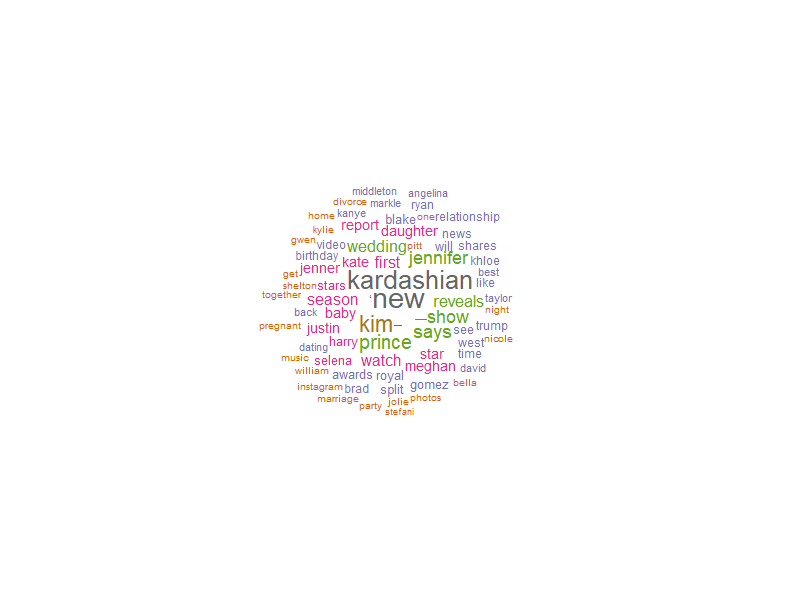
\includegraphics[width=11.11in]{wordcloud}

\begin{Shaded}
\begin{Highlighting}[]
\FunctionTok{wordcloud}\NormalTok{(}\AttributeTok{words =}\NormalTok{ d}\SpecialCharTok{$}\NormalTok{word, }\AttributeTok{freq =}\NormalTok{ d}\SpecialCharTok{$}\NormalTok{freq, }\AttributeTok{min.freq =} \DecValTok{1}\NormalTok{, }\AttributeTok{max.words =} \DecValTok{75}\NormalTok{, }\AttributeTok{random.order =} \ConstantTok{FALSE}\NormalTok{, }\AttributeTok{rot.per =} \DecValTok{0}\NormalTok{, }\AttributeTok{scale =} \FunctionTok{c}\NormalTok{(}\FloatTok{2.4}\NormalTok{, }\FloatTok{0.35}\NormalTok{), }\AttributeTok{colors =} \FunctionTok{brewer.pal}\NormalTok{(}\DecValTok{8}\NormalTok{, }\StringTok{"Dark2"}\NormalTok{))}
\FunctionTok{dev.off}\NormalTok{()}
\end{Highlighting}
\end{Shaded}

\begin{verbatim}
## pdf 
##   2
\end{verbatim}

\begin{Shaded}
\begin{Highlighting}[]
\FunctionTok{library}\NormalTok{(igraph)}
\end{Highlighting}
\end{Shaded}

\begin{verbatim}
## 
## Attaching package: 'igraph'
\end{verbatim}

\begin{verbatim}
## The following objects are masked from 'package:stats':
## 
##     decompose, spectrum
\end{verbatim}

\begin{verbatim}
## The following object is masked from 'package:base':
## 
##     union
\end{verbatim}

\begin{Shaded}
\begin{Highlighting}[]
\NormalTok{file\_path }\OtherTok{\textless{}{-}} \StringTok{"results.csv"}
\NormalTok{data }\OtherTok{\textless{}{-}} \FunctionTok{read.csv}\NormalTok{(file\_path)}
\NormalTok{data }\OtherTok{\textless{}{-}} \FunctionTok{subset}\NormalTok{(data, tournament }\SpecialCharTok{==} \StringTok{"AFC Asian Cup"}\NormalTok{)}
\NormalTok{data }\OtherTok{\textless{}{-}} \FunctionTok{data.frame}\NormalTok{(}\AttributeTok{winner =} \FunctionTok{ifelse}\NormalTok{(data}\SpecialCharTok{$}\NormalTok{home\_score }\SpecialCharTok{\textgreater{}}\NormalTok{ data}\SpecialCharTok{$}\NormalTok{away\_score, data}\SpecialCharTok{$}\NormalTok{home\_team, data}\SpecialCharTok{$}\NormalTok{away\_team), }\AttributeTok{loser =} \FunctionTok{ifelse}\NormalTok{(data}\SpecialCharTok{$}\NormalTok{home\_score }\SpecialCharTok{\textgreater{}}\NormalTok{ data}\SpecialCharTok{$}\NormalTok{away\_score, data}\SpecialCharTok{$}\NormalTok{away\_team, data}\SpecialCharTok{$}\NormalTok{home\_team), }\AttributeTok{date =} \FunctionTok{as.Date}\NormalTok{(data}\SpecialCharTok{$}\NormalTok{date))}
\FunctionTok{library}\NormalTok{(dplyr)}
\end{Highlighting}
\end{Shaded}

\begin{verbatim}
## 
## Attaching package: 'dplyr'
\end{verbatim}

\begin{verbatim}
## The following objects are masked from 'package:igraph':
## 
##     as_data_frame, groups, union
\end{verbatim}

\begin{verbatim}
## The following objects are masked from 'package:stats':
## 
##     filter, lag
\end{verbatim}

\begin{verbatim}
## The following objects are masked from 'package:base':
## 
##     intersect, setdiff, setequal, union
\end{verbatim}

\begin{Shaded}
\begin{Highlighting}[]
\NormalTok{y }\OtherTok{\textless{}{-}}\NormalTok{ data }\SpecialCharTok{\%\textgreater{}\%} \FunctionTok{group\_by}\NormalTok{(winner, loser) }\SpecialCharTok{\%\textgreater{}\%} \FunctionTok{summarise}\NormalTok{(}\AttributeTok{weight =} \FunctionTok{n}\NormalTok{(), }\AttributeTok{.groups =} \StringTok{\textquotesingle{}drop\textquotesingle{}}\NormalTok{)}
\NormalTok{y }\OtherTok{\textless{}{-}}\NormalTok{ y }\SpecialCharTok{\%\textgreater{}\%} \FunctionTok{arrange}\NormalTok{(winner, loser) }\SpecialCharTok{\%\textgreater{}\%} \FunctionTok{filter}\NormalTok{(}\SpecialCharTok{!}\FunctionTok{duplicated}\NormalTok{(}\FunctionTok{paste}\NormalTok{(}\FunctionTok{pmin}\NormalTok{(winner, loser), }\FunctionTok{pmax}\NormalTok{(winner, loser))))}
\NormalTok{net }\OtherTok{\textless{}{-}} \FunctionTok{graph.data.frame}\NormalTok{(y, }\AttributeTok{directed =} \ConstantTok{TRUE}\NormalTok{)}
\FunctionTok{V}\NormalTok{(net)}\SpecialCharTok{$}\NormalTok{label }\OtherTok{\textless{}{-}} \FunctionTok{V}\NormalTok{(net)}\SpecialCharTok{$}\NormalTok{name}
\FunctionTok{V}\NormalTok{(net)}\SpecialCharTok{$}\NormalTok{degree }\OtherTok{\textless{}{-}} \FunctionTok{degree}\NormalTok{(net, }\AttributeTok{mode =} \StringTok{"all"}\NormalTok{)}
\NormalTok{net }\OtherTok{\textless{}{-}} \FunctionTok{delete.vertices}\NormalTok{(net, }\FunctionTok{V}\NormalTok{(net)[}\FunctionTok{degree}\NormalTok{(net, }\AttributeTok{mode =} \StringTok{"out"}\NormalTok{) }\SpecialCharTok{\textless{}} \DecValTok{5}\NormalTok{])}
\FunctionTok{png}\NormalTok{(}\StringTok{"network\_graph.png"}\NormalTok{, }\AttributeTok{width =} \DecValTok{800}\NormalTok{, }\AttributeTok{height =} \DecValTok{600}\NormalTok{)}
\NormalTok{knitr}\SpecialCharTok{::}\FunctionTok{include\_graphics}\NormalTok{(}\StringTok{"network\_graph.png"}\NormalTok{)}
\FunctionTok{plot}\NormalTok{(net, }\AttributeTok{layout =}\NormalTok{ layout\_with\_fr, }\AttributeTok{vertex.color =} \FunctionTok{rainbow}\NormalTok{(}\FunctionTok{length}\NormalTok{(}\FunctionTok{V}\NormalTok{(net))), }\AttributeTok{vertex.size =} \FunctionTok{log}\NormalTok{(}\FunctionTok{V}\NormalTok{(net)}\SpecialCharTok{$}\NormalTok{degree }\SpecialCharTok{+} \DecValTok{1}\NormalTok{) }\SpecialCharTok{*} \DecValTok{6}\NormalTok{, }\AttributeTok{edge.arrow.size =} \FloatTok{0.3}\NormalTok{, }\AttributeTok{vertex.label.cex =} \FloatTok{0.8}\NormalTok{, }\AttributeTok{vertex.label.color =} \StringTok{"black"}\NormalTok{, }\AttributeTok{main =} \StringTok{"AFC Asian Cup Network Graph"}\NormalTok{)}
\FunctionTok{dev.off}\NormalTok{()}
\end{Highlighting}
\end{Shaded}

\begin{verbatim}
## pdf 
##   2
\end{verbatim}

\begin{Shaded}
\begin{Highlighting}[]
\NormalTok{knitr}\SpecialCharTok{::}\FunctionTok{include\_graphics}\NormalTok{(}\StringTok{"network\_graph.png"}\NormalTok{)}
\end{Highlighting}
\end{Shaded}

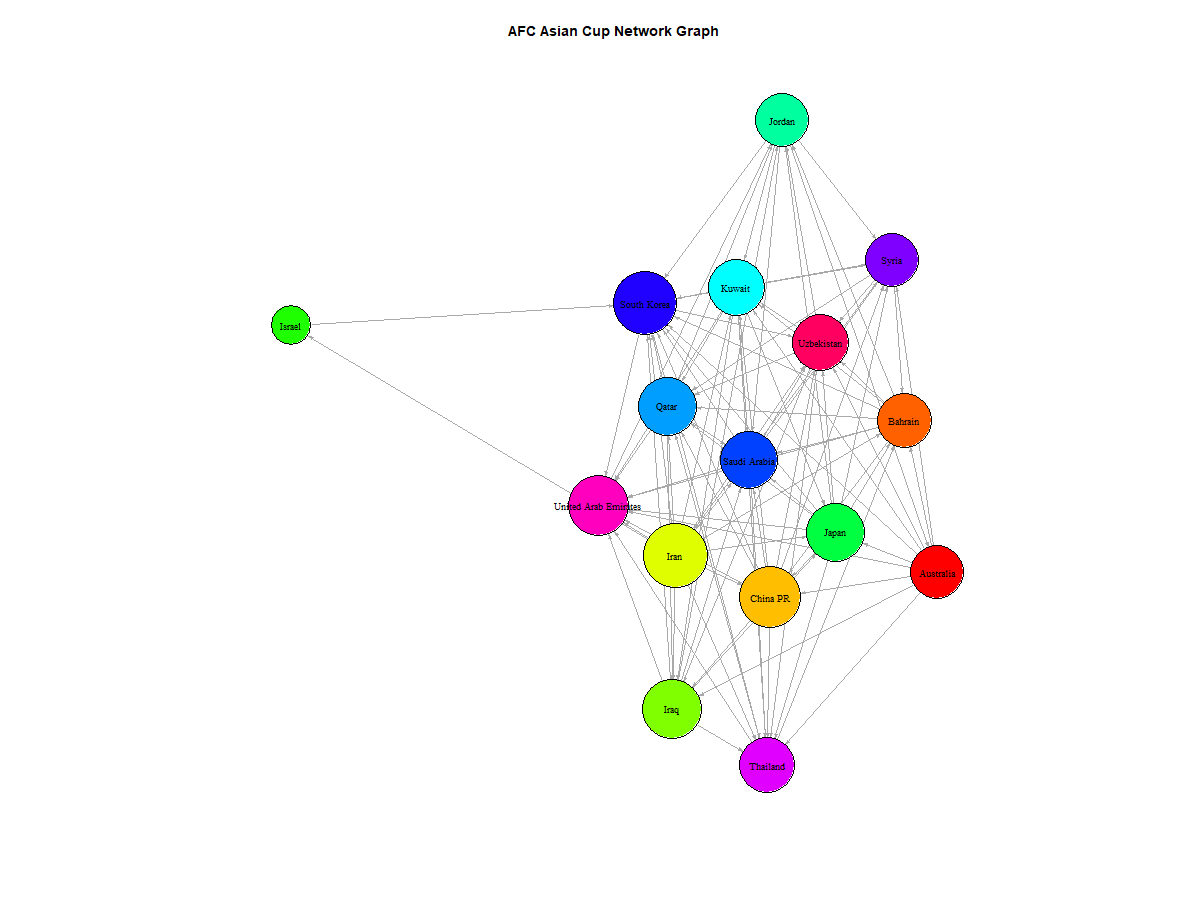
\includegraphics[width=11.11in]{network_graph}

\end{document}
